
\chapter{Deployment}
	The analysis results are targeted at decision-makers such as financial analysts and strategists. The clustering results can be part of a in-depth financial analysis, and provide a very broad overview on spending.
	
	The questions this overview should answer are:
	\begin{itemize}
		\item Which spending categories exist?
		\item How does the spending divide onto the categories?
		\item Which magnitude exists between the different amounts spent?
	\end{itemize}
	
	The results of an analysis are often summarized using a business intelligence visualization tool. In this case, the analysis is visualized using Tableau.
\begin{figure}[h!]
	\centering
	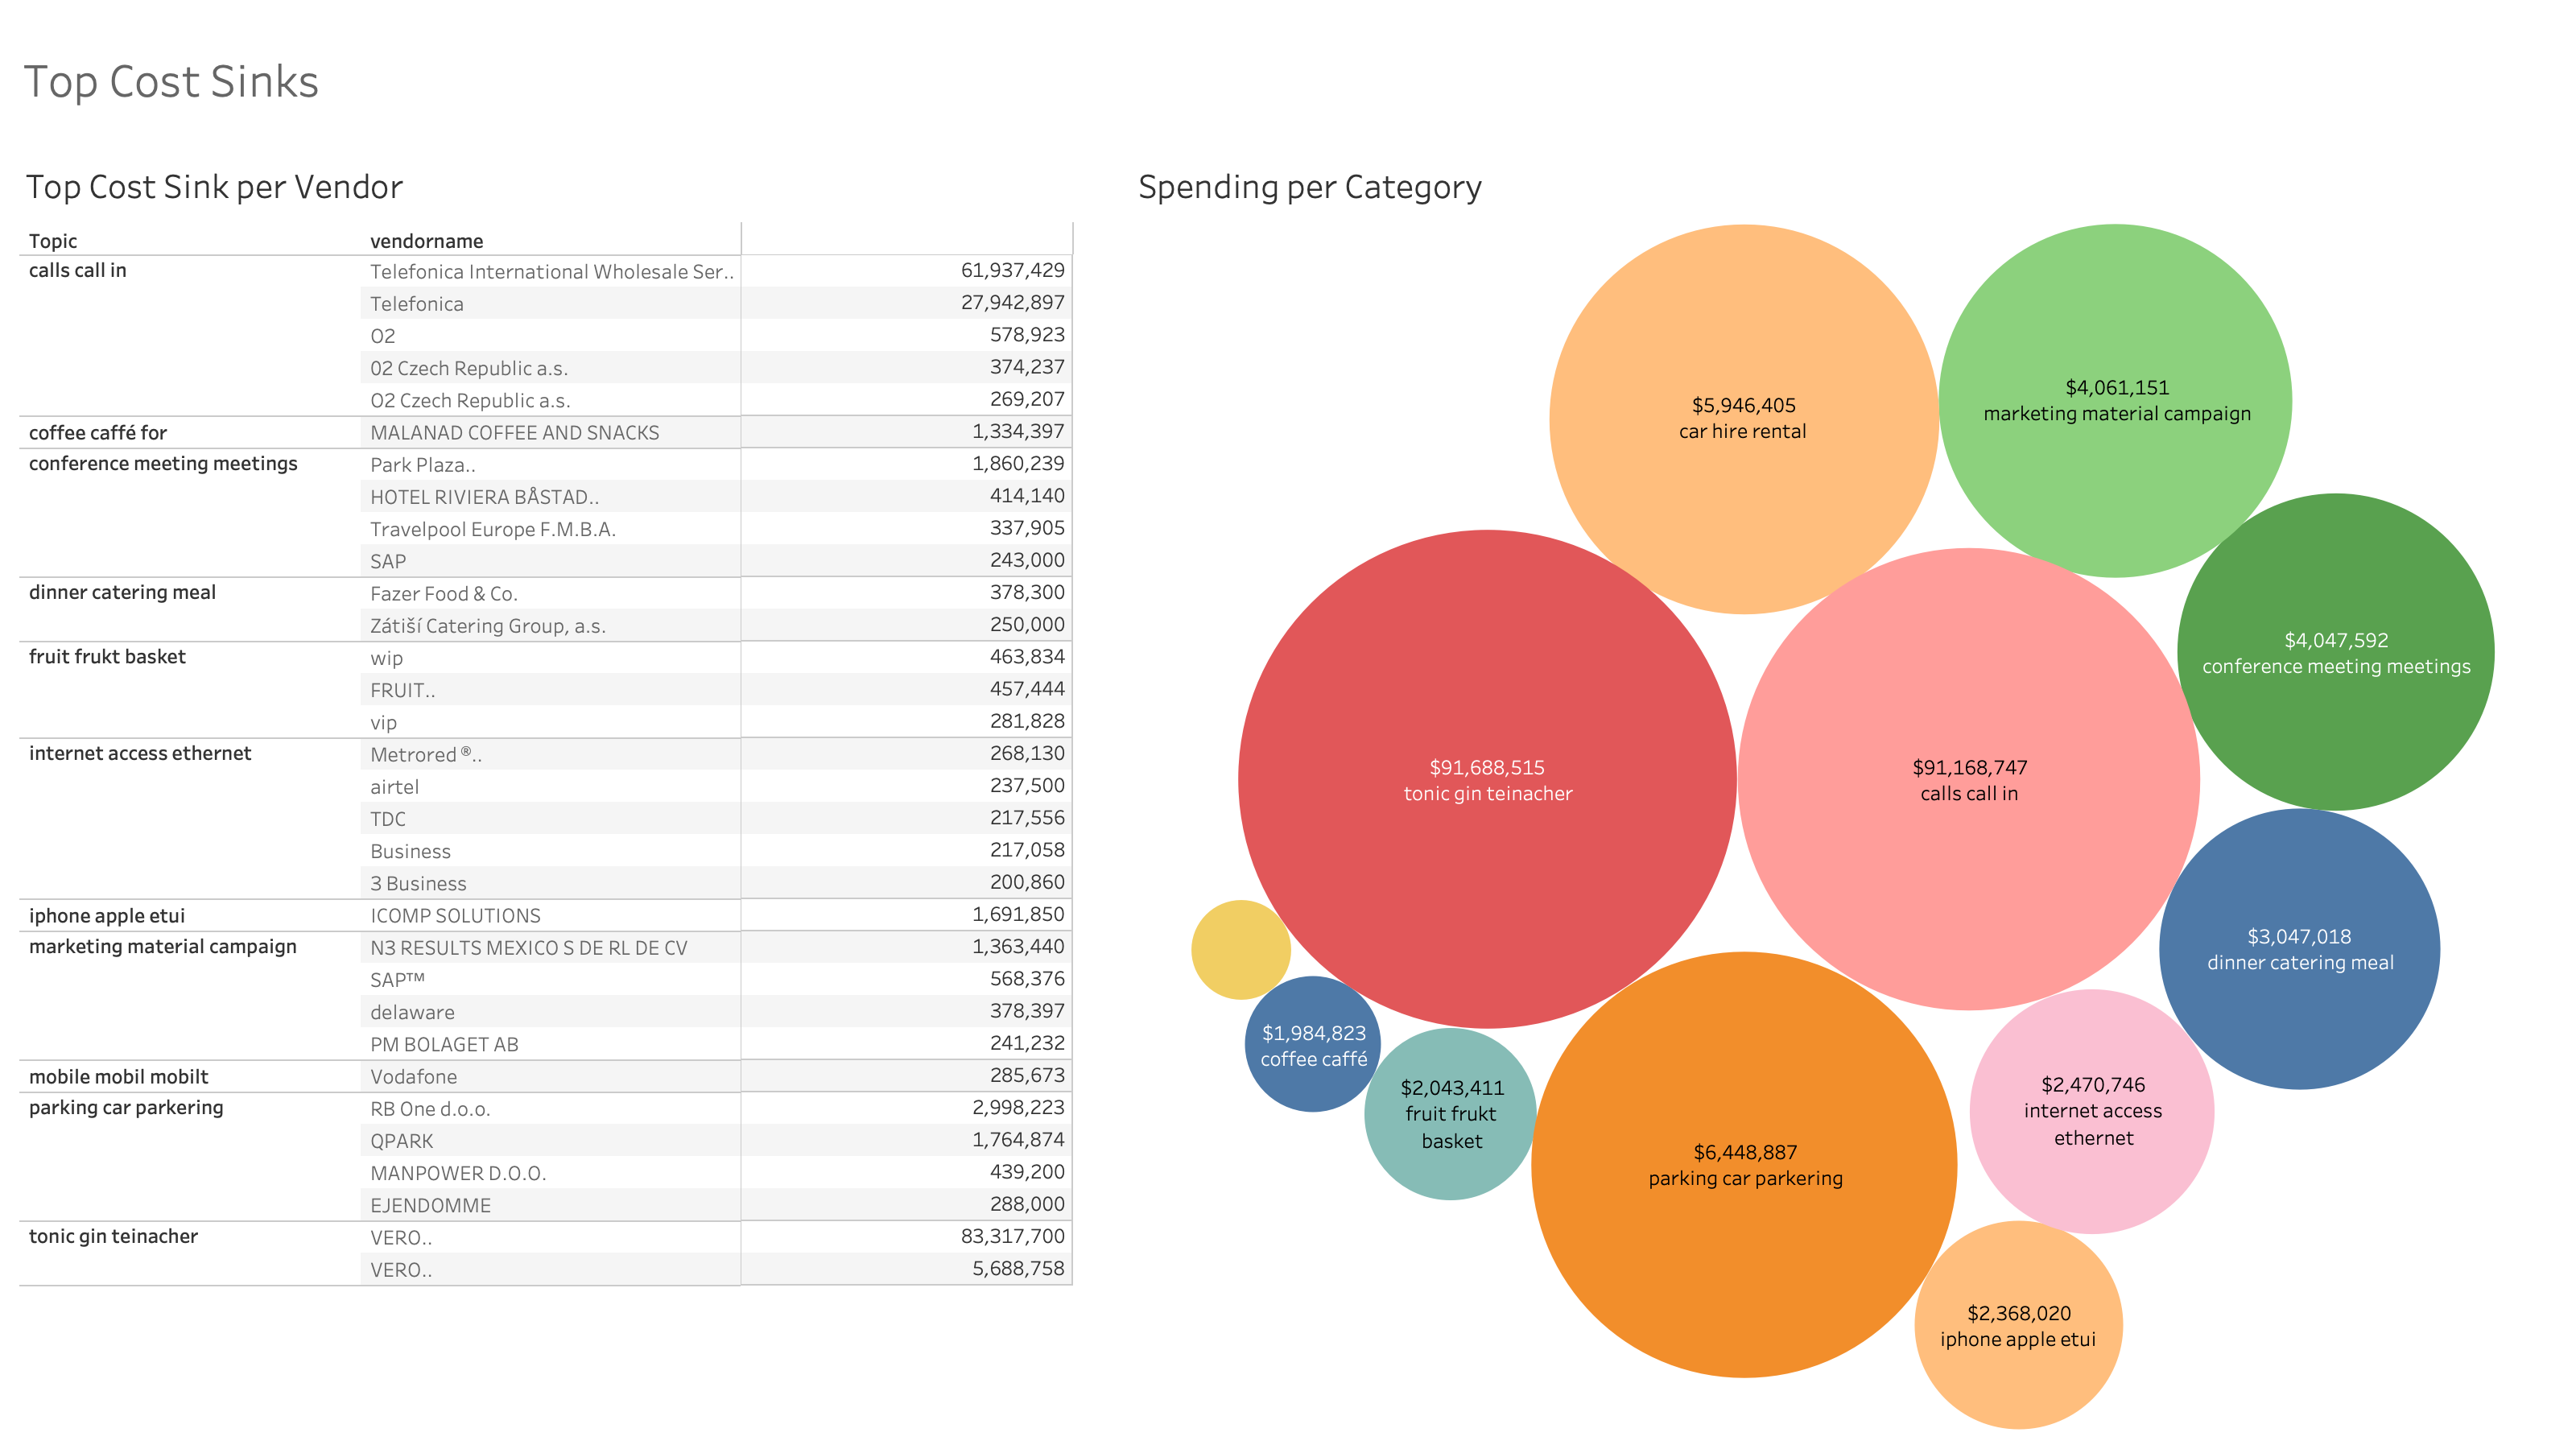
\includegraphics[
	width=\linewidth,
	angle=90]{Bilder/deployment/bubble.png}
	\caption{Tableau Dashboard: Overview on the largest Spending Categories}
	\label{fig:dashboard-bubble}
\end{figure}

\begin{figure}[h!]
	\centering
	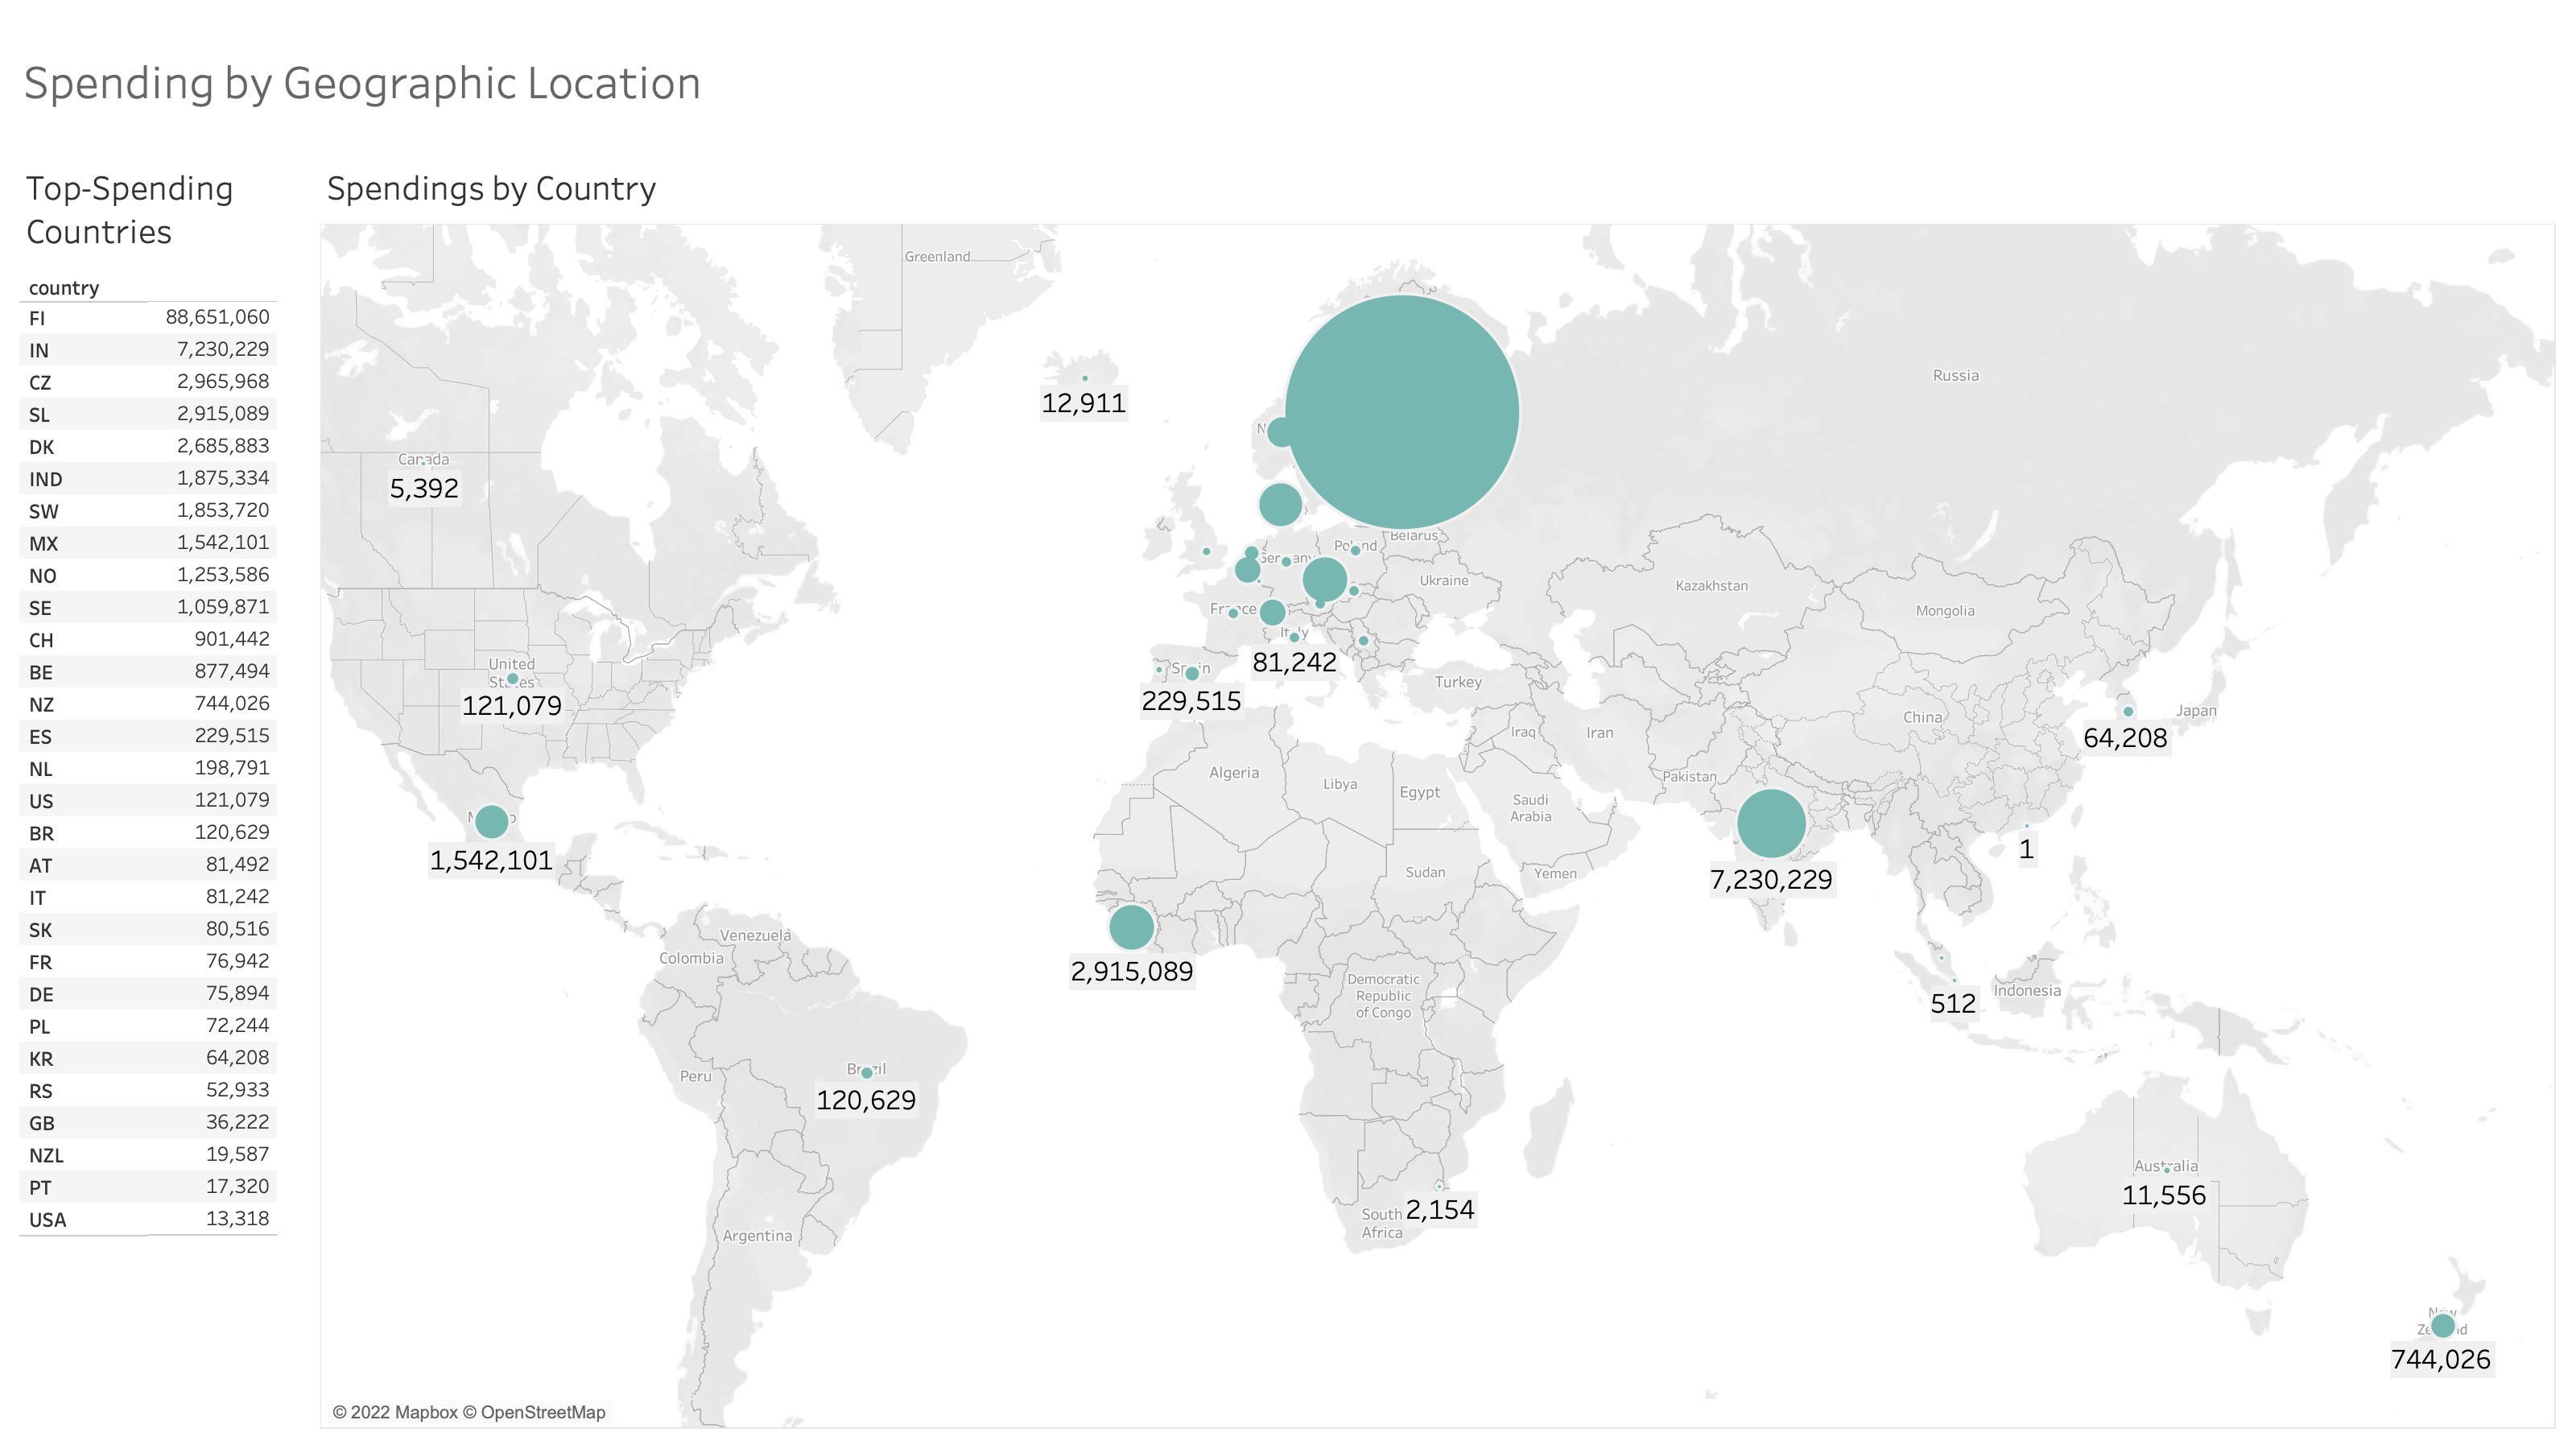
\includegraphics[width=\linewidth,
	angle=90]{Bilder/deployment/world.png}
	\caption{Tableau Dashboard: Overview on the largest Spending Categories}
	\label{fig:dashboard-world}
\end{figure}

	The dashboard answers all questions. First, it shows the big picture of spending. Additional insights are in the tool tips of each bubble in the chart. The table on the right hand side provides a convenient ranking of the different spending categories.
	
